\newpage

\section{项目简介}

\subsection{工作内容简介}

Slow6502 是我们小组编写的一个 MOS Technologies 6502 微处理器和兼容系统的通用模拟器。Slow6502 可以模拟 1 MHz NMOS 6502 或 CMOS 65C02、32KB RAM、16KB ROM,并且可以模拟 MOS 6551 Motorola 6850 ACIA、MOS 6522 VIA 和 6545 CRTC 等外设,从而模拟一个完整的系统。此外,Slow6502 还支持 MOS 65C02 等 6502 的变体,以及不同内存和外设地址布局的设备。

Slow6502 提供加载程序和加载 ROM 等功能,使得众多6502的程序可以在其上执行。此外,如果用户只有针对特定平台的 ROM 或者二进制文件,则其可以轻松地通过修改 Slow6502 的 machine 部分的源码来添加不同外设和内存布局的设备,从而运行对应的二进制文件。

该项目由 Java 8 写成,实现了共 30 个设计模式,包括 23 个 GoF 设计模式和 7 个 非 GoF 设计模式。

\begin{figure}[htb]
  \centering
  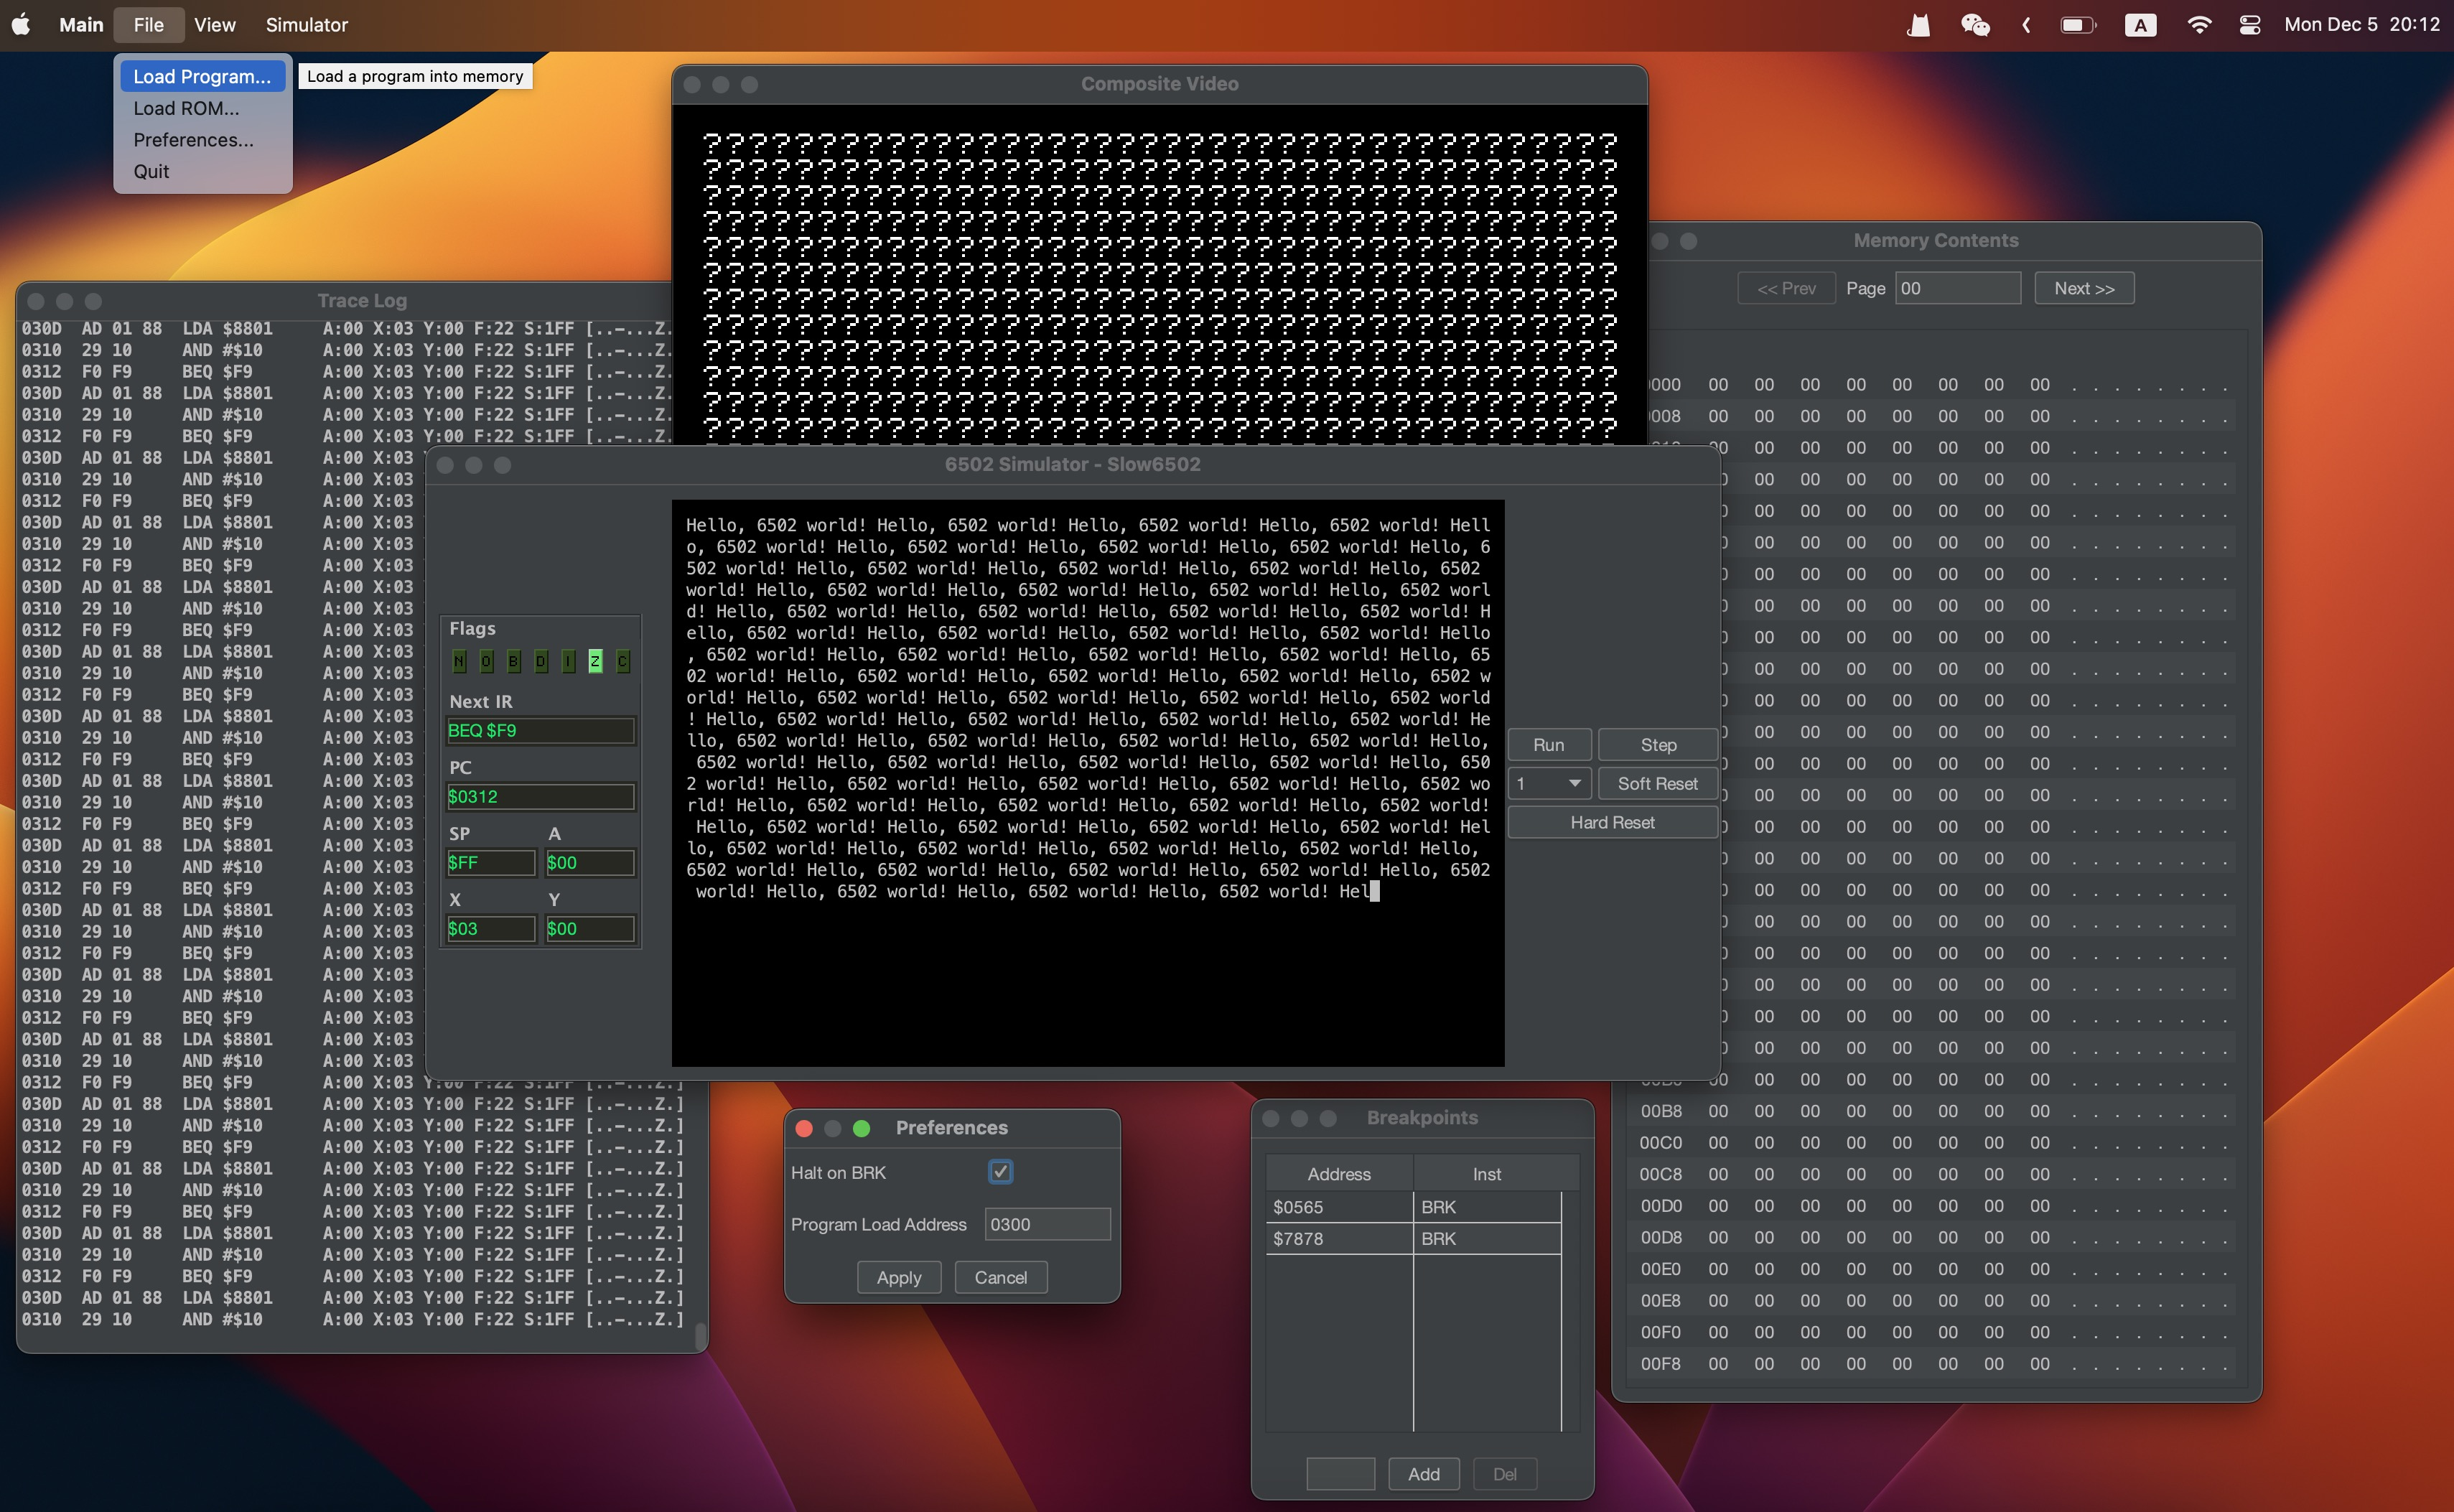
\includegraphics[width=0.9\textwidth]{image/Slow6502UI.jpg}
  \caption{Slow6502 界面概览}
\end{figure}

\newpage
\subsection{选题背景}

\paragraph{关于 6502} MOS Technology 6502 是一款 8 位微处理器,最多可以寻址64KB内存,拥有两个通用寄存器,一个累加器和一个栈寄存器。

\begin{figure}[htb]
  \centering
  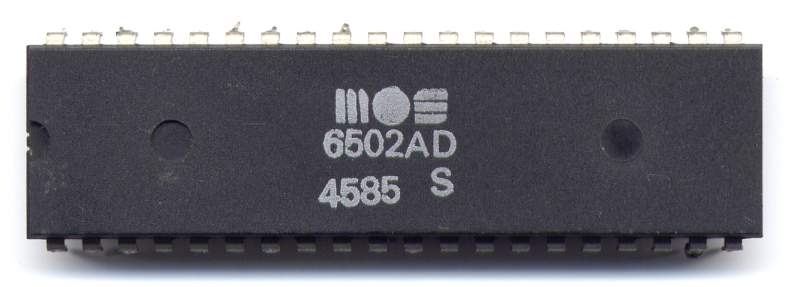
\includegraphics[width=0.7\textwidth]{image/MOS_6502AD_4585_top.jpeg}
  \caption{DIP-40 塑料封装的 MOS 6502 处理器(85 年 45 周产)}
\end{figure}

MOS 6502 是由 Chuck Peddle 领导的 MOS Technology 团队设计的。设计团队曾在摩托罗拉从事摩托罗拉6800项目; 6502 本质上是该设计的简化、更便宜和更快的版本。

在 1975 年推出时,6502 是市场上价格最低的微处理器,遥遥领先。它最初的售价不到 6800 或 Intel 8080 等大公司竞争设计成本的六分之一。它的推出导致整个处理器市场的价格迅速下降。它与 Zilog Z80 一起引发了一系列项目,导致了 80 年代初期的家用电脑革命。

1980 年代和 90 年代初期流行的视频游戏机和家用电脑,例如 Atari 2600、Atari 8 位系列、Apple II、Nintendo Entertainment System、Commodore 64、Atari Lynx、BBC Micro 等,使用 6502 或 6502 的变体基本设计。 6502 推出后不久,MOS Technology 被 Commodore International 彻底收购,Commodore International 继续向其他制造商销售微处理器和许可。在 6502 的早期,它由 Rockwell 和 Synertek 二次采购,后来授权给其他公司。

时至今日,依然有诸多爱好者仿制6502和用它搭建怀旧电脑。即使和同时代的英特尔8080, 摩托罗拉6800相比,它也是平平无奇的:3510个晶体管,56个指令,最高3 MHz的主频。看似平庸的6502依靠着仅有对手六分之一的价格、亲民的姿态、和车库文化交融的理念构成了美国60到70一代年轻计算机爱好者的集体记忆。

\paragraph{MOS 6502 和我国的计算机产业} 得益于 MOS 6502 廉价的设计思路和良好的生态,其可能是第一个能广泛被中国学生们用到的CPU。

著名的中华学习机 CEC-I 就“使用”了 MOS 6502 作为其 CPU。这款由电子工业部计算机与信息局组织,清华大学主持联合设计,电子部六所、国营 734 厂、陕西省计算机厂以及华明计算机有限公司参与研制的机型是 Apple II 的仿制品。

\begin{figure}[htb]
  \centering
  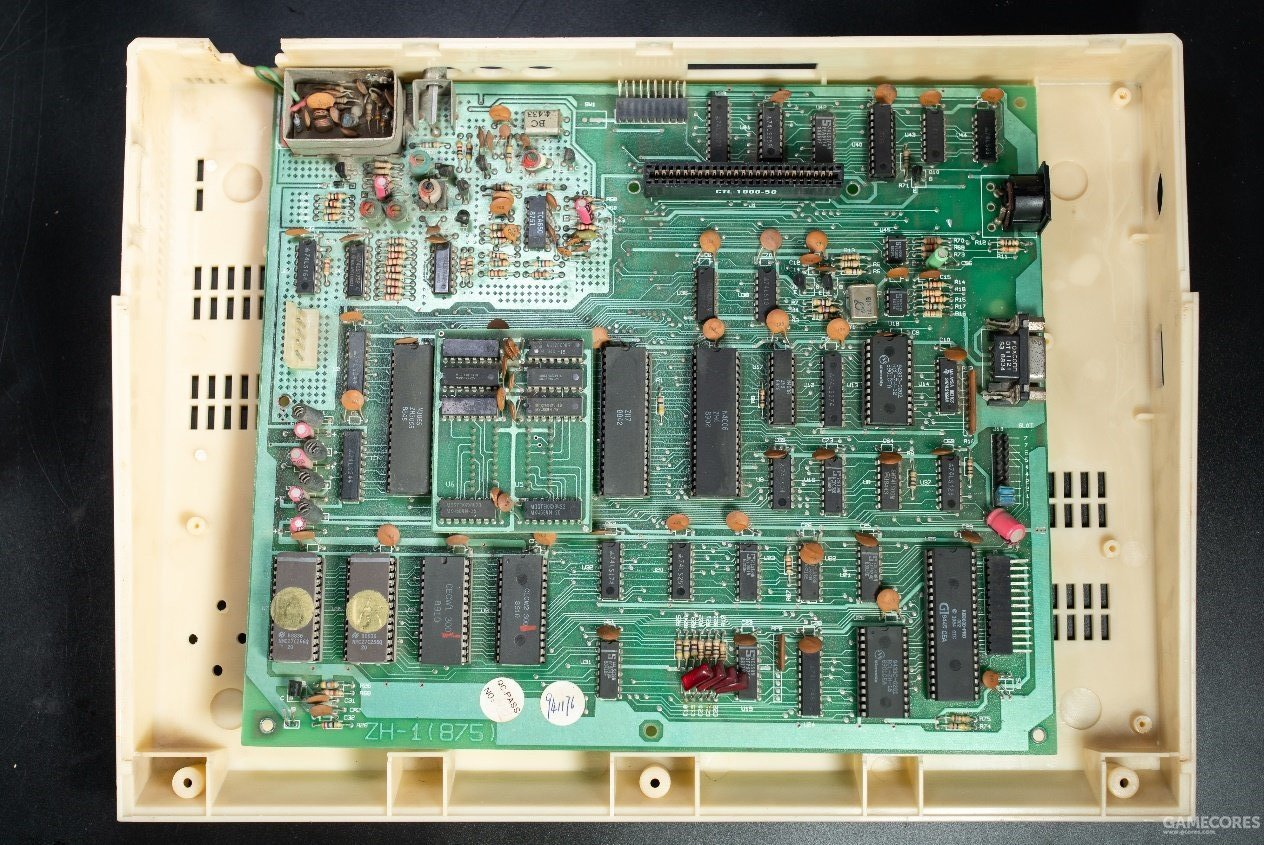
\includegraphics[width=0.7\textwidth]{image/CIC1.jpeg}
  \caption{一块中华学习机的主板,可见中间 DPI-40 封装的 CPU}
\end{figure}

这款机器是芯片级仿制的 Apple II 计算机,如果你拆开机器,会发现除了某些早期试验型号,里面并没有使用 MOS 6502 CPU。而是一些标着 ZH-6、ZH-7、ZH3065 的芯片,而这些芯片就是对 Apple II 内部芯片的完全仿制,包括 MOS 6502。在那个靠 decapping 技术就可以了解 CPU 内部构造的年代,这款机器的诞生虽然不能说是容易的,但也是很神奇了。而且这款机器内置了汉卡和 80 列卡。这两款卡在一般 Apple II 上是需要单独购买的,有了这两块卡,不但可以显示和输入汉字,还可以显示更多的列数,让一行显示的字符数变多一倍,由于中文通常要占用两个字符宽度,这对于中文使用是非常重要的。

这款机器的价格大约是当时中产阶级家庭一年的收入,虽然并不能做到家用,但是很多学校都有一两台这个机器。至少让很多人从小接触到了计算机。

除了中华学习机外,上世纪末红遍大江南北的FC兼容机/小霸王学习机们和后来几乎人手一台的文曲星都采用了6502 CPU。从诞生至今的40多年来,6502对个人电脑和家用游戏主机行业产生了极其深刻的影响,无数人的人生因此而改变。虽然小霸王和文曲星早已经不再流行,各类 NES 上的游戏也逐渐被人遗忘,但直到现在,6502仍被运用于数以亿计的工业监测和控制计算机当中,为我们服务。
